%% PRÄAMBEL

% -- Dokumentenklasse
\documentclass[
	% Schriftgröße
	11pt,
	% Papierformat
	a4paper,
	% Seitenverteilung
	oneside,
	% Sprache
	ngerman
	]{article}


\usepackage[ngerman]{babel}

% -- Schriftart Latin Modern verwenden (Vektor)
%\usepackage{lmodern}

% -- Schriftart Roboto Condensed verwenden (Vektor)
\usepackage[sfdefault]{roboto}

% -- Meta-Daten
\newcommand{\mytitle}{Pr\"aventive messtechnische Abbildung typischer Fertigungsabweichungen}
\newcommand{\myname}{Jan Doant}

% -- Seitenränder
\usepackage[left=30mm,right=20mm,top=25mm,bottom=20mm]{geometry}

% -- Zeilenabstand
\usepackage{setspace}
\makeatletter
\newcommand{\MSonehalfspacing}{%
	\setstretch{1.44}%  default
	\ifcase \@ptsize \relax % 10pt
	\setstretch {1.448}%
	\or % 11pt
	\setstretch {1.399}%
	\or % 12pt
	\setstretch {1.433}%
	\fi
}
\newcommand{\MSdoublespacing}{%
	\setstretch {1.92}%  default
	\ifcase \@ptsize \relax % 10pt
	\setstretch {1.936}%
	\or % 11pt
	\setstretch {1.866}%
	\or % 12pt
	\setstretch {1.902}%
	\fi
}
\makeatother
\MSonehalfspacing

% -- Deutsche Absatztrennung
\usepackage{parskip}

%% -- Gestaltung Kopf- und Fußzeile
% -- Kopfzeile
\usepackage{fancyhdr}
\addtolength{\headheight}{3pt}
\lhead{\mytitle}
% -- Fußzeile
\lfoot{\myname}
\cfoot{}
\rfoot{Seite~\thepage}  

%% -- deutsches Sprachpaket
% -- deutsche Silbentrennung
\usepackage[ngerman]{babel}
% -- Umlaute
\usepackage[utf8]{inputenc}
\usepackage[T1]{fontenc}
% -- deutsche Anführungszeichen
\usepackage[babel,german=quotes]{csquotes}

% -- Mathematikpakete
\usepackage{amsmath}
\usepackage{amsfonts}
\usepackage{esvect}
% -- Vektordarstellung
\usepackage{esvect}

% -- Grafikpaket
\usepackage{graphicx}

% -- Verweise 
% -- Verweise werden im Dokument klickbar
\usepackage[pdfpagelabels]{hyperref}
% -- Einfärben von Verweisen
\usepackage[dvipsnames,svgnames,x11names,hyperref]{xcolor}
\hypersetup{
	% Meta-Informationen, die in der PDF-Datei gespeichert werden
	pdfauthor={\myname},
	pdftitle={\mytitle},
	% Einfärben der Schrift
	colorlinks = true,
	% Farbe von Verknüpfungen im Text 
	linkcolor=[RGB]{63 81 181},
	% Farbe von Quellenverweisen
	citecolor= [RGB]{76 175 80},
	% Farbe von URLs
	urlcolor=[RGB]{0 76 153},
}

% -- Verweise automatisieren
%\usepackage{cleveref}
\usepackage{varioref}
\usepackage{prettyref}

% -- prettyref-Befehl konfigurieren
\newrefformat{sec}{Abschnitt \vref{#1}}
\newrefformat{fig}{Abbildung \vref{#1}}
\newrefformat{tab}{Tabelle \vref{#1}}
\newrefformat{lis}{Codebeispiel \vref{#1}}
\newrefformat{eq}{Formel \vref{#1}}


% -- Anzeigen der verwendeten Labels (nur im Dev-Modus verwenden)
\usepackage[
	% Label wird am inneren Rand angezeigt
	inner,
	% blendet Label aus, wenn final aktiv 			 
	final			 
	]{showlabels}

% -- Bibliografiestil
\usepackage[
	% Literaturverzeichnis wird in der Reihenfolge, in der die Referenzen genannt werden sortiert
	sorting=none,
	% keine Angabe der URL 		
	url=false,
	% Übersicht Biblatex-Styles:
	% https://de.sharelatex.com/learn/Biblatex_bibliography_styles 			
	style=ieee,
	% keine Angabe der ISBN 			
	isbn=false,
	% Datumsangabe nur für das Erscheiningsjahr
	date=year,
	% maximal 6 Namen in der Literaturliste
	maxbibnames=6,
	% mindestens 3 Namen in der Literaturliste    
	minbibnames=3,
	% Verwendung von biber.exe
	backend=biber
	]{biblatex}

% -- Pfad zur .bib-Datei
\addbibresource{bib/lit.bib}

% -- Tabellenpaket
\usepackage{tabularx}
\renewcommand{\arraystretch}{1.5}

% -- Verzeichnisse zum Inhaltsverzeichnis hinzufügen
\usepackage[
	% Inhaltsverzeichnis selbst nicht im Inhaltsverzeichnis aufführen 
	nottoc
	]{tocbibind}

% -- TikZ
\usepackage{tikz}

% -- Listings
\usepackage{listings}
\renewcommand{\lstlistingname}{Codebeispiel}
\lstdefinestyle{customc}{
	belowcaptionskip=1\baselineskip,
	breaklines=true,
	xleftmargin=2cm,
	language=[x86masm]Assembler,
	showstringspaces=false,
	basicstyle=\ttfamily,
	keywordstyle=\bfseries\color{green!40!black},
	commentstyle=\itshape\color{purple!40!black}
}

%% DOKUMENT
\begin{document}
	
% -- Titelseite
\pagenumbering{Alph}
\pagestyle{empty}
\begin{titlepage}
	
\begin{figure}[htbp]
	\begin{minipage}{0.19\textwidth}
		% \textwidth bezieht sich nun auf die Minipage
		\includegraphics[width=\textwidth]{img/logo_tuc.pdf}
	\end{minipage}
	% Auffüllen des Zwischenraums
	\hfill
	% minipage mit Text
	\begin{minipage}{0.6\textwidth} 
		\begin{center}	
			Technische Universität Chemnitz\\
			Fakultät Maschinenbau\\
			Professur Fertigungsmesstechnik
		\end{center}
	\end{minipage}
	\hfill
	\begin{minipage}{0.19\textwidth} 
		% \textwidth bezieht sich nun auf die Minipage
		
\includegraphics[width=\textwidth]{img/logo_fmt.pdf}
	\end{minipage}
\end{figure}
	
	
	\vspace*{1cm}
		
		\begin{center}	
		
		\vspace{1.5cm}
		
		{\huge\textbf{Bachelorarbeit}}
		
		\vspace{1.5cm}
		
		{\large Arbeitstitel:}\\
		{\large\textbf{\mytitle}}
		
		\vspace{1.5cm}
		
		Betreuer: M. Sc. Robert Hofmann\\
		Prüfer: Univ.-Prof. Dr.-Ing. Sophie Gröger		
		
		\vfill
		
			
		
	\end{center}
	
	\begin{flushleft}
		Name: Jan Doant\\		
		E-Mail: jan.doant@s2017.tu-chemnitz.de\\
		Studiengang: Bachelor Maschinenbau (7. Semester)\\
		Matrikelnummer: 461311\linebreak
		
		
		Eingereicht am: 06.06.2018
		
	\end{flushleft}
	
	
\end{titlepage}
\newpage

% -- Inhaltsverzeichnis
\pagestyle{empty}
%%Anzahl der maximal aufgeführten Gliederungspunkte
\setcounter{tocdepth}{3}
\tableofcontents
\newpage

%% --Sandbox
%\pagestyle{fancy}
%\section{Sandbox}

\subsection{Sandbox--Zitierung}

Das ist zu eine zu zitierende Textstelle \cite{Hesse2016}.
Und hier ist noch ein Zitat.\cite{Vogt2003}
Wenn man was aus diesem Buch zitieren soll. \cite{Quarteroni2005}

\subsection{Sandbox--Grafiken einbinden}

\begin{figure}[htbp] 
  \centering
     \includegraphics[width=0.7\textwidth]{img/logo_tuc.pdf}
  \caption{Logo der Technischen Universität Chemnitz}
  \label{fig:Bild1}
\end{figure}

\newpage

\newpage


\subsection{Sandbox--Referenzierung}

Ich beziehe mich auf \prettyref{fig:Bild1}.
%\newpage

\pagenumbering{arabic}
\pagestyle{empty}
\section{Aufgabenstellung}

Alle realen Fertigungsverfahren erzeugen gewisse charakteristische geometrische Abweichungen von der Nenngestalt, die zum Beispiel einem zeitlichen Trend oder einer zufälligen Auftretenswahrscheinlichkeit folgen. Ursache für diese Abweichungen sind dem jeweiligen Fertigungsverfahren innewohnende, teils unvermeidliche Erscheinungen. Zu diesen gehören zum Beispiel der Verschleiß des Werkzeugs oder äußere Schwingungen. 

Die beherrschte Vorhersage solcher Abweichungen ist bedeutend zur Absicherung der Produktqualität über die gesamte Produktionsstückzahl. Die Kenntnis über die sich wahrscheinlich einstellenden Ist-Abweichungen der Nenngestalt ist wichtig für verschiedene Prozesse der Fertigungsmesstechnik, wie zum Beispiel zur Definition der Messstrategie (Messpunktmuster, Messpunktanzahl, etc.). 

Ziel der Abschlussarbeit ist einerseits die umfassende Zusammenstellung und Kategorisierung charakteristischer geometrischer Fertigungsabweichungen. Darauf aufbauend ist ein geeignetes Werkzeug zu generieren, um die zu erwartenden Abweichungen durch eine erzeugte Punktewolke darzustellen.
Das geschieht, indem die vorhandene Soll-Geometrie durch einen geeigneten Algorithmus mit den erarbeiteten typischen Fertigungsfehlern beaufschlagt werden können. Dafür wird die Umsetzung mittels MATLAB oder einer geeigneten CAD-Software vorgeschlagen. 

\paragraph{Teilaufgaben}

\begin{itemize}
	\item Recherche und Katalogisierung von charakteristischen geometrischen Abweichungen, die aus realen Fertigungsverfahren hervorgehen können
	\item Erarbeitung eines Werkzeugs zur Erzeugung von erwartbaren Messpunktwolken durch die Beaufschlagung der Soll-Geometrie mit geometrischen Fertigungsabweichungen, zum Beispiel mittels MATLAB oder CAD
	\item Zusammenstellung der Erkenntnisse und Erarbeitung eines Ausblicks  
\end{itemize}
\newpage



% -- Einführung / Motivation
\pagestyle{fancy}
\section{Einführung}
\label{sec:einfuehrung}

\subsection{Hallo}







\newpage

% -- Grundlagen / Stand der Technik
\pagestyle{fancy}
\section{Grundlagen}

\subsection{Oberflächenabweichungen und -unvollkommenheiten}

Um die Qualität einer technischen Oberfläche beurteilen zu können, ist es zunächst unerlässlich, verschiedene standardisierte Begriffe zu definieren. Dazu geben sowohl DIN 4760 als auch DIN EN ISO 8785 diverse Bezeichnungen vor, welche die möglichen auftretenden Oberflächenunvollkommenheiten voneinander abgrenzen und ordnen sollen.

\subsubsection{Wirkliche Oberfläche}

DIN 4760 definiert den Begriff der Wirklichen Oberfläche als die tatsächliche, den betrachteten Gegenstand von seinem Umgebungsmedium trennende Oberfläche. Für die Messtechnik ist diese Gestalt allerdings nicht in voller Gänze zu erfassen. Aus diesem Grund werden weitere Begriffe benötigt, um die Wirkliche Oberfläche zu abstrahieren und für die Messtechnik verfügbar zu machen. 

\subsubsection{Istoberfläche}

Als Istoberfläche bezeichnet die oben beschriebene Norm das messtechnisch erfasste Abbild der Wirklichen Oberfläche eines Formelementes. Dabei ist festzuhalten, dass hier von einer bereits vereinfachten Oberfläche zu sprechen ist. Abhängig von Messverfahren, Messparametern, Messplan und Messabfolge ergeben sich für verschiedene Messungen auch unterschiedliche Istoberflächen des Objektes. Dies ist bei der Betrachtung und Analyse einer Istoberfläche stets zu beachten. Natürlich wirken sich auch systematische und zufällige Messfehler auf die Gestalt der Istoberfläche aus. Um von der messtechnisch erfassten Gestalt des Bauteils auf dessen Gestaltabweichungen schließen zu können, ist der nachfolgende Begriff der Geometrischen Oberfläche unerlässlich. 

\subsubsection{Geometrische Oberfläche}

Als Geometrische Oberfläche wird in DIN 4760 die ideale Form des betrachteten Objektes definiert. Sie wird auch als Nennform bezeichnet und ist durch die jeweiligen technischen Zeichnungen oder andere technische Unterlagen, wie zum Beispiel 3D-CAD-Informationen festgeschrieben. Da kein Fertigungsprozess fehlerfrei abläuft, ist es unmöglich, diese Idealgeometrie in der Realität zu fertigen. Allerdings ist es mit Hilfe der technischen Dokumente möglich, zulässige Abweichungen von der Idealgeometrie festzulegen. Vielmehr dient diese Beschreibung in der Messtechnik als Referenz, um die im folgenden Abschnitt behandelten Gestaltabweichungen überhaupt erst erfassbar zu machen.
     
\subsubsection{Gestaltabweichungen}

Als Gestaltabweichungen werden in der beschreibenden Norm die Gesamtheit aller Abweichungen der messtechnisch erfassten Istoberfläche von der idealen geometrischen Oberfläche bezeichnet. Grundlage für das Vorhandensein von Gestaltabweichungen sind mannigfaltig und werden in den folgenden Abschnitten weiter ausgeführt. Grundsätzlich ist festzustellen, dass unterschieden wird zwischen solchen Abweichungen, die nur durch Betrachtung des gesamten Objektes feststellbar sind, und Abweichungen, die nur durch Analyse eines Ausschnittes der Oberfläche erkennbar werden (siehe Abb.\ref{fig:din4760_1}). Dazu werden die Gestaltabweichungen in 6 verschiedenen Ordnungen klassifiziert. 


\begin{figure}[h]
	\centering
	\includegraphics[width=0.5\linewidth]{img/DIN_4760_1}
	\caption[Ausschnitt aus der Istoberfläche zur Beurteilung der Gestaltabweichung]{Ausschnitt aus der Istoberfläche}
	\label{fig:din4760_1}
\end{figure}

Als Gestaltabweichungen 1. Ordnung werden in DIN 4760 jene Gestaltabweichungen beschrieben, die, wie weiter oben bereits angeschnitten, bei der Beurteilung der gesamten Istoberfläche ersichtlich werden. Abweichungen dieser Kategorie werden als Formabweichungen bezeichnet. Darunter zählen beispielsweise Geradheits-, Ebenheits- und Rundheitsabweichungen. Diese Art der Abweichungen begründet die Norm in fehlerhaften Führungen der bearbeitenden Maschine, Durchbiegung von Werkzeug oder Werkzeugmaschine, falscher Einspannung des Werkstückes, Verschleiß oder Härteverzug.

Die 2. Ordnung der Gestaltabweichungen wird unter dem Begriff Welligkeit geführt. Es handelt sich dabei um periodisch wiederholt auftretende Gestaltabweichungen der gemessenen Oberfläche eines untersuchten Formelements. Als wellig definiert die Norm DIN 4760 Abweichungen, bei denen das Verhältnis von Wellenabständen zur Wellentiefe generell zwischen 1000 : 1 und 100 : 1 liegt. Es handelt sich also um relativ niederfrequente Wellen mit einer verhältnismäßig niedrigen Amplitude. Als grundlegende Ursachen für die Entstehung von welligen Formen nennt die Norm sowohl außermittige Einspannung des Werkstücks als auch Form- und Laufabweichungen des Werkzeugs und Schwingungen der Werkzeugmaschine und des Werkzeugs.

Die Gestaltabweichungen 3. bis 5. Ordnung werden als Rauheit bezeichnet. Sie sind nur durch Betrachtung eines Oberflächenausschnitts des Objektes zu erkennen. Rauheitsabweichungen kehren entweder regelmäßig oder unregelmäßig wieder. Sie sind gekennzeichnet durch ein Verhältnis der Abstände zur Tiefe zwischen 100 : 1 und 5 : 1. Es handelt sich also im Vergleich zum im vorherigen Abschnitt beschriebenen Welligkeitsphänomen um hochfrequentere Abweichungen der Oberfläche. 
Innerhalb der Klasse der Rauheitsabweichungen lassen sich verschiedene Ausprägungen beschreiben. So unterscheidet die Norm Rillen (4. Ordnung), Riefen, Schuppen, Kuppen (5. Ordnung) und Oberflächenrauheit, welche durch die Gefügestruktur hervorgerufen wird (6. Ordnung).
Diese Kategorien unterscheiden sich in Frequenz und Amplitude ihrer Form (siehe Abb. *Todo*). Außerdem lassen sich verschiedene Ursachen für ihr Auftreten finden. 

Rillen werden durch die Form der Werkzeugschneide sowie aufgrund des eingestellten Vorschubes und der Schnittbewegung des Werkzeuges hervorgerufen.
Riefen, Schuppen und Kuppen sind Oberflächenunvollkommenheiten, deren Gründe im Prozess der Spanbildung zu finden sind. Des Weiteren lassen sie sich beispielsweise durch Werkstoffverformung beim Strahlen oder Knospenbildung bei galvanischer Behandlung erklären. 

Rauheiten, welche durch die Gefügestruktur des Werkstoffes verursacht werden, sind durch Kristallisationsvorgänge oder Veränderungen der Oberfläche beispielsweise durch chemische oder korrosive Vorgänge entstanden. Sie bilden zusammen mit der 6. Ordnung der Gestaltabweichungen, welche durch den Gitteraufbau des Materials zu erklären sind, die nicht mehr durch Messverfahren ermittelbaren Gestaltabweichungen. 

Das bedeutet, dass in der Istoberfläche für gewöhnlich eine Struktur zu erkennen ist, die durch Überlagerung der Gestaltabweichungen 1. bis 4. Ordnung verursacht wird. 

\subsubsection{Oberflächenunvollkommenheiten}

Zusätzlich zu den in DIN 4760 aufgeführten Gestaltabweichungen werden in DIN EN ISO 8785 Oberflächenunvollkommenheiten erläutert. In der Norm werden diese als "`Element, Unregelmäßigkeit oder Gruppe von Elementen und Unregelmäßigkeiten der Wirklichen Oberfläche, die unbeabsichtigt oder zufällig durch die Bearbeitung, Lagerung oder Funktion der Oberfläche entstanden sind"' definiert. Es wird dabei unterschieden zwischen nach innen orientierten (Vertiefung), nach außen gerichteten (Buckel), kombinierten und stellenweisen Oberflächenunvollkommenheiten. Kombinierte Oberflächenunvollkommenheiten enthalten sowohl Anteile von Vertiefungen als auch Buckeln. Stellenweise Unvollkommenheiten besitzen eine kaum messbare Erhöhung bzw. Vertiefung. 

In \prettyref{fig:din-en-8785-beispiele} sind einige Beispiele für jede genannte Kategorie der Oberflächenunvollkommenheiten zu finden. 

\begin{figure}[h]
	\centering
	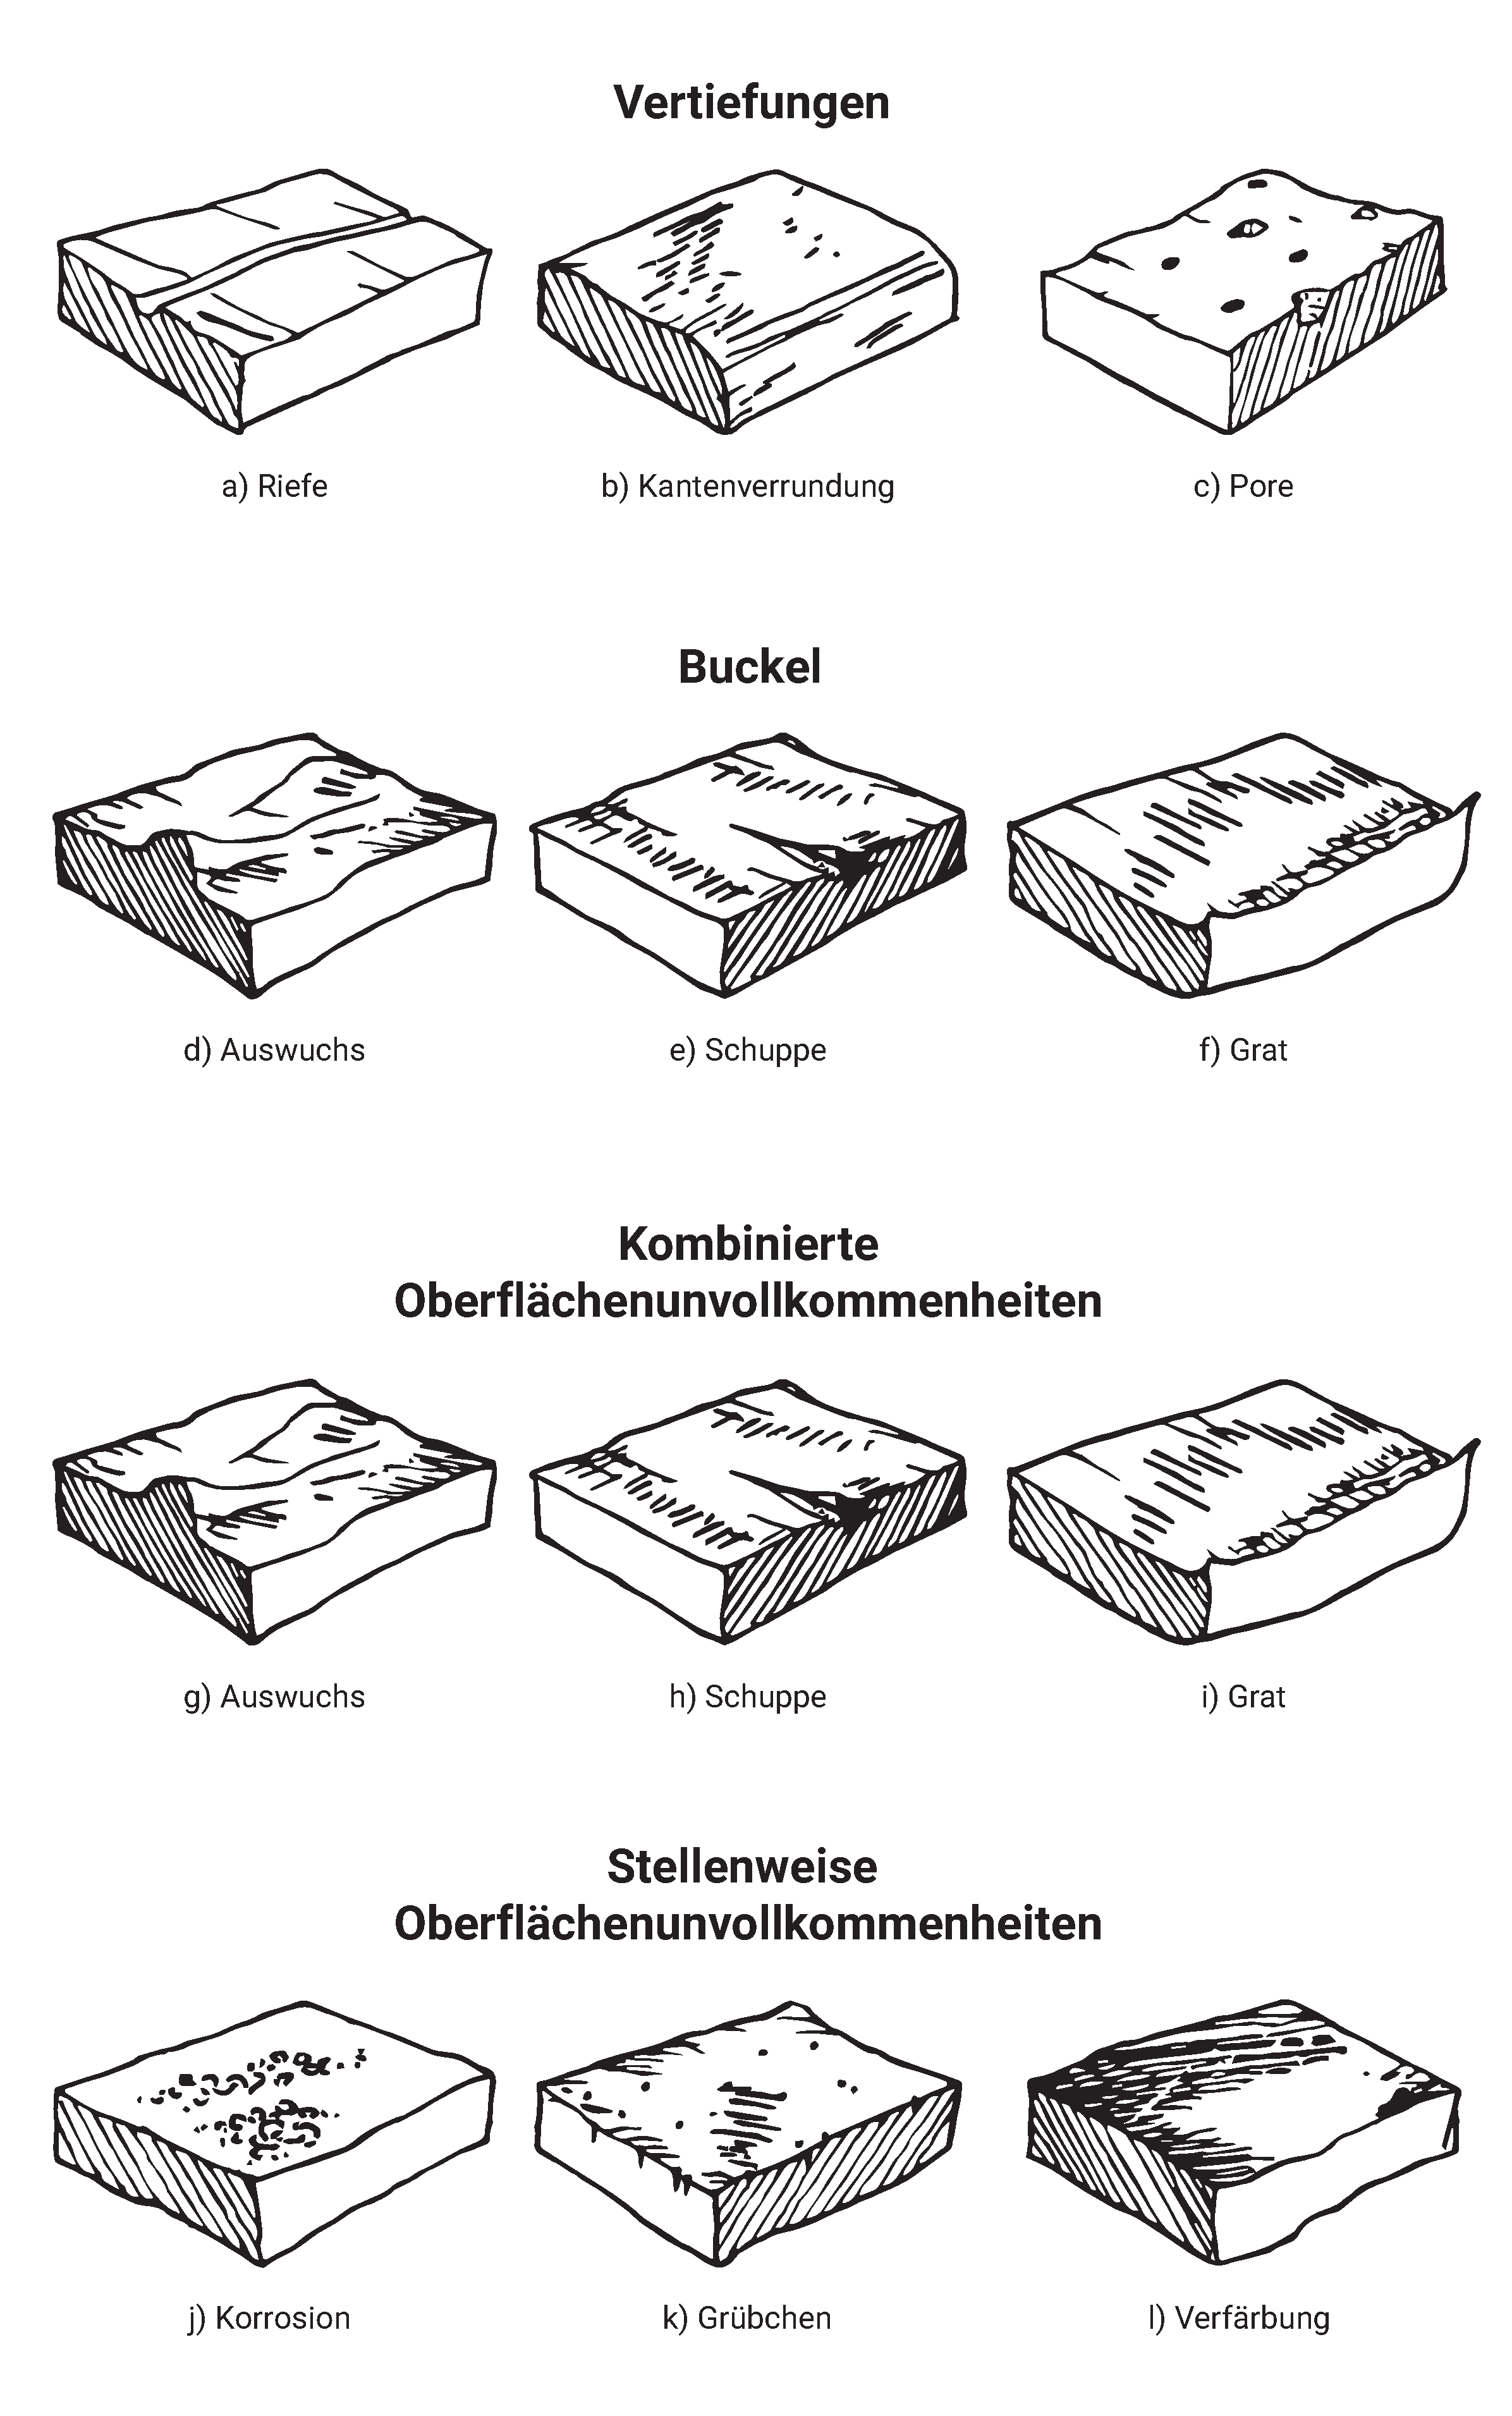
\includegraphics[width=0.7\linewidth]{img/din_en_8785_beispiele}
	\caption[DIN EN ISO 8785 - Oberflächenunvollkommenheiten]{DIN EN 8785 - Oberflächenunvollkommenheiten}
	\label{fig:din-en-8785-beispiele}
\end{figure}









 






          




\subsection{Typische Abweichung verschiedener spanender Fertigungsvefahren}

\subsubsection{Ursachen für Fertigungsabweichungen}

Jedes Bauteil, welches in einem Fertigungsverfahren hergestellt wird entspricht in seiner Realgestalt nicht der in den Fertigungsunterlagen (Technische Zeichnung oder CAD-Model) festgehaltenen Idealgeometrie. Es sind durch verschiedene Einflüsse stets Abweichungen von der Geometrischen Oberfläche des Objektes festzustellen. Dies hat nach [Denkena] verschiedene Ursachen, die im Werkstück selbst, dem bearbeitenden Werkzeug, der Werkzeugmaschine oder Fertigungsumgebung liegen. 

So werden als Ursachen für Fertigungsabweichungen, die durch das Werkzeug bestimmt werden bereits vorhandene Form- und Lagetoleranzen des Rohteils, Festigkeitsunterschiede der abzuspanenden Teile, Auslösung bzw. Einbringung von Eigenspannungen in das Werkstück und örtlich und zeitlich veränderliche Temperaturfelder im Bauteil genannt.
Es ist festzuhalten, dass Wärmeeinbringung am Werkstück vor allem Formfehler zur Folge hat. Bei zylindrischen Bauteilen zeigen sich diese hauptsächlich in axialer Richtung, wegen inhomogener elastischer Erwärmung.

Weiterhin hat auch das bearbeitende Werkzeug einen sehr großen Einfluss auf die wirkliche Geometrie des Bauteils. Hier sind besonders die Nachgiebigkeit des Werkzeugs bzw. Werkzeughalters, die Lageabweichung des Werkzeugs beim Werkzeugwechsel sowie der Verschleiß des Werkzeugs zu nennen. Dabei hat der Werkzeugverschleiß einen maßgeblichen Einfluss auf die Maß- und Formgenauigkeit. Werkzeugverschleiß führt zu Schneidenversatz, dies wiederum begründet die Fehler, die die Maßhaltigkeit betreffen. Die Formabweichungen sind in den durch den Werkzeugverschleiß auftretenden höheren Schneidkräften bedingt. Diese führen zusammen mit der Nachgiebigkeit Werkzeugmaschine zum auftreten dieser Abweichungen.

Der Einfluss der bearbeitenden Maschine liegt in ihrer Nachgiebigkeit im Kraftfluss und ihrer thermischen Wirkung. So kommt es zu geometrischen Abweichungen und thermisch bedingten Verformungen während des Bearbeitungsprozesses. Ungenauigkeiten in den Führungen der Werkzeugmaschine führen über die kinematischen Kette der Maschine zu sich fortpflanzenden geometrischen Fehlern im Bauteil [Neugebauer] 

Auch die Umgebung der Maschine wirkt natürlich auf die Werkstückqualität ein. So führen externe Wärmequellen, Änderungen der Umgebungstemperatur oder eine Veränderung der Kühlschmierung zu Abweichungen am Werkstück. Zählt man den Bearbeiter des Bauteils zu den Umgebungsfaktoren hinzu, ergeben sich auch durch systematische oder zufällige menschliche Fehler in der Einrichtung und Überwachung des Bearbeitungsprozesses, Einflüsse auf die Formgestalt des Bauteils. 

Es ist festzuhalten, dass ein komplexes System an Einflussfaktoren auf das Werkstück einwirken, die sich gegenseitig beeinflussen können. Es ist nicht möglich, ohne detaillierte Kenntnis aller Faktoren bereits im Vorfeld konkret vorherzusagen, welche Abweichungen bei einem Fertigungsverfahren zu erwarten sind. Durch Erfahrungswerte lassen sich allerdings typische Abweichungen für die einzelnen Fertigungsverfahren beschreiben. 

\subsubsection {Fertigungsabweichungen beim Drehen}

Beim Fertigungsverfahren Drehen sind, je nach konkretem Drehverfahren, unterschiedliche Maßtoleranzen zu erreichen. So sind laut [Dietrich.2014] beim Schlichtdrehen Toleranzen von IT7 bis IT8 realistisch, beim Feinschlichten können unter optimalen Drehbedingungen sogar Genauigkeiten von IT6 umgesetzt werden. Das deckt sich mit den Angaben nach [Denkena.2011] wonach mit konventionellen Drehmaschinen Maßabweichungen von IT6 bis IT7 realisierbar sind. Ergänzend dazu werden mögliche Rundheitsabweichungen auf konventionellen Drehmaschinen von von weniger als 2,5µm, Zylindrizitätsabweichungen von weniger als 2µm und gemittelte Rautiefen $R_{z}$ von 2 bis 6µm beschrieben. 

Außerdem wird die mögliche Fertigungsgenauigkeit von Präzisionsdrehmaschinen genannt. Dabei werden Maßabweichungen im Bereich von IT5 bis IT6, Rundheitsabweichungen von 0,2µm, Zylindrizitätsabweichungen von weniger als 0,1µm sowie eine gemittelte Rauhtiefe $R_{z}$ von 0,5µm erreicht. Dies ist also ein deutlich genaueres Verfahren, was bei der Betrachtung der zu erwartenden Abweichungen unbedinngt in Erwägung gezogen werden muss. 

Die theoretische Oberflächenrauheit einer drehend hergestellten Oberfläche lässt sich laut [Dietrich.2014] und [Paucksch.2008] mit der Formel 

\begin{equation*}
	R_{t}=\frac{f^{2}}{r_{\epsilon}}
\end{equation*}

berechnen. In dieser Formel beschreibt $r_{\epsilon}$ den Eckenradius und $f$ den Vorschub des Werkzeugs in axialer Richtung. Die Vorschubgeschwindigkeit hat demnach einen quadratischen Einfluss auf die theoretische Oberflächenrauheit und gibt diese maßgeblich vor. Mit zunehmender Nutzungsdauer des Werkzeuges steigt dessen Verschleiß wobei sich somit der Betrag des Eckenradius stets ändert. Dies resultiert laut oben genannter Formel in einer Veränderung der Oberflächengüte des bearbeiteten Geometrieelements. 

Drehende Verfahren weisen eine starke gerichtete Bearbeitungsrichtung auf, weshalb durchweg gerichtete, rillige Oberflächen entstehen. Diese gerichteten Oberflächen weisen in der Regel quer zur Schnittrichtung größere Rauheiten als in Schnittrichtung auf.[Denkena]
Diese Rillen sind stark geprägt von der Form und dem Verschleißzustand des Drehmeißels sowie der Vorschubbewegung. [Paucksch.2008]
Weiterhin ist die Oberflächenrauheit geprägt von der Zerspanbarkeit des Werkstoffes. Eine gute Zerspanbarkeit ermöglicht geringe Fehler in der Form und Oberflächengüte des Bauteils. Werkstoffe mit einer homogenen Gefügeausbildung erreichen eine höhere Arbeitsgüte einfacher als Werkstücke mit Fehlstellen (z.B. Lunker oder Porositäten).

Wie alle Verfahren erzeugt auch das Drehen erfahrungsgemäß typische Fehler am Werkstück, die konkreten Ursachen zugeordnet werden können. Dies ermöglicht, den Rückschluss vom Fehler auf die Ursache und ermöglicht eine Anpassung der Prozessparameter um eine höhere Arbeitgenauigkeit zu steuern. 

Ungenügende Maßgenauigkeit lässt sich zum Beispiel über einen zu hohen Verschleiß des Werkzeuges erklären. Mit übermäßigem Verschleiß wird der Schneidkantenversatz des Drehmeißels zu groß, was eine kontrollierte Einstellung der Oberflächenrauheit erschwert. Eine weitere Ursache für zu hohe Maßabweichungen kann weiterhin in einer Durchbiegung des eingespannten Werkstückes liegen. Dies resultiert aus zu hohen Passivkräften bei der Zerspanung (zu hohe Schnittiefe oder Werkzeugvorschub), fehlender Abstützung schlanker Werkstücke oder einem zu hohen Einstellwinkel $\kappa$ des Werkzeuges. [Schönherr]

Ein weiterer Fehler, der sich bei drehend hergestellten Bauteilen finden lässt ist die Unrundheit des Profils außerhalb der vorgegebenen Toleranzen. Ein Grund dafür liegt in der übermäßigen Durchbiegung des Bauteils aus den oben genannten Gründen. Außerdem wirken sich eine ungenaue, außermittige Zentrierung, Längsführungen oder Haupspindellagerungen mit zu viel Spiel und elastische Verformungen des Werkstückes durch zu hohe Spannkräfte negativ auf die Rundheit des Bauteils aus.[Dietrich.2014], [Schonherr.2002] 

Bei Drehteilen lassen sich weiterhin wellige Oberflächen feststellen. Die ergibt sich aus Schwingungen der Drehmaschine und damit auch des Werkzeuges im Eingriff durch zu hohes Spiel in den Führungen der Maschine. Außerdem führen eine zu falsche Werkzeugeinspannung und zu hohe Schnittleistungen zum Einbringen von zusätzlichen Schwingungen in die Werkzeugmaschine, was die Bildung welliger Oberflächen begünstigt. [Dietrich.2014] 

Rattermarken am Werkstück entstehen aufgrund eines instabilen Werkzeugs (Auskraglänge zu groß, Schaftquerschnitt zu gering oder instabile Einspannung), zu hohen Passivkräften bei der Bearbeitung, einem zu hohen Freiflächenverschleiß oder einer ungenügenden Schneidkantenschärfe des Werkzeugs, beispielsweise wegen einer Beschichtung dessen. [Schonherr.2002]

Eine konische Form des angestrebten zylindrischen Bauteils entsteht laut [Dietrich] aufgrund einer nicht fluchtenden Anordnung von Drehachse der Maschine und der Achse der Spitze des Reitstocks. 

Kratzer auf der Oberfläche eines Drehteils lassen sich auf Oxidationsverschleiß der Nebenschneide des Werkzeugs oder auf den Kontakt mit Spänen zurückführen, welche die fertig gedrehte Oberfläche beschädigen. [Schonherr.2002] 

\subsubsection {Fertigungsabweichungen beim Bohren}

Beim Fertigungsverfahren Bohren sind verschiedene Maßtoleranzen und Rautiefen zu erreichen. Auch beim Bohren sind die Werte stark von dem Bohrverfahren und den Prozessparametern abhängig.
\prettyref{tab:bohrungsqualitaet} stellt den Sachverhalt anschaulich dar.

\begin{table}[h]	
	
	\begin{tabularx}{\columnwidth}{|X|c|c|l|}	
		
		
		\hline
		\textbf{Verfahren}&\textbf{Maßtoleranz}&\textbf{Rautiefe $R_{t}$ in µm}&\textbf{Oberflächenqualität}\\
		\hline
		Bohren ins Volle&IT12&80&Schruppen\\
		\hline
		Aufbohren mit Wendelsenkern&IT11&20&Schlichten\\
		\hline
		Senken mit Flach- und Form\-senkern&IT9&12&Schlichten\\
		\hline
		Reiben&IT7&8&Feinschlichten\\
		\hline
		Ausdrehen mit Ausdrehmeißel oder mehrschneidigem Bohrkopf&IT7&8&Feinschlichten\\
		\hline
		Ausdrehen mit Hartmetallschneiden und sehr kleinem Spanungsquerschnitt&IT7&4&Feinschlichten\\
		\hline	
		
	\end{tabularx}
	
	\caption{Maßtoleranzen und Rautiefen verschiedener Bohrverfahren (Quelle: Todo)}
	\label{tab:bohrungsqualitaet}

\end{table}

Des Weiteren beschreibt [Schoenherr] die Abhängigkeit der erreichbaren Genauigkeiten vom Material des Bohrers. So sind mit HSS-Spiralbohrern Toleranzen von IT12, mit Vollhartmetall-Spiralbohrern Toleranzen von IT9 und mit geradgenutetem Vollhartmetallbohrer Toleranzen von IT7 herstellbar. 

Generell ist aber zu sagen, dass ein Bohren ins Volle mit einem Wendelbohrer stets eine Schruppbearbeitung darstellt. Das heißt es ist keine hochgenaue Fertigung möglich. Viel bessere Genauigkeiten lassen sich mit Reiben, Senken, Feinbohren und Ausdrehen erzielen. [Schonherr.2002]

Die Formgenauigkeit einer Bohrung wird hauptsächlich durch deren Rundheit und Geradheit beschrieben. Mangelnde Formgenauigkeit kann verschiedene Ursachen haben. Dazu zählen eine nicht ausreichen hohe Steifigkeit von Werkzeugmaschine, Werkzeug und der Werkzeugaufnahme. Weiterhin wirken sich eine schlechte Zentrierung beim Anschnitt, ungleichmäßiges Schneiden aller Hauptschneiden des Bohrers und zu hohe Belastungen (Vorschub- und Schnittkräfte) negativ auf die Formhaltigkeit der Bohrung aus. Positiv können sich hingegen die Verwendung geradgenuteter oder rechtsgedrallter Bohrer und eine gute Spanbildung (Spanformung, Spanbruch, Spanabfuhr) niederschlagen. 

Von Werkzeugen verursachte Asymmetrien unterscheiden sich deutlich von werkstückbedingten Asymmetrien. Dadurch entstehen typische Bohrfehler.

Durch ungünstige Werkzeuge zu begründende Fehler bohrend hergestellter Flächen sind beispielsweise Überweite und Konizität des Geometrielements. Dabei sind nach [Paucksch] vor allem durch Anschlifffehler erzeugte asymmetrische Werkzeuge ursächlich. Diese sind charakterisiert durch Hauptschneidenlängenunterschiede, Einstellwinkeldifferenzen, Spitzenlängenabweichungen und Außermittigkeit der Werkzeugquerschneide.
Überweite kommt dabei am häufigsten vor. [Winkler] nennt neben dem ungünstigen Anschliff des Bohrers außerdem den Einsatz falscher Bohrerdurchmesser sowie den übermäßig langen und damit verschleißreichen Einsatz von Bohrern als weitere Gründe für eine Überweite der Bohrung. 
Weiterhin kann es bei stumpfen Bohrern zur Ausbildung einer Wulst an der Oberseite bei gleichzeitiger Gratbildung an der Unterseite kommen. Ebenfalls durch einen stumpfen Bohrer werden sehr raue Bohrungswandungen hervorgerufen. 
Hat das Werkzeug eine schlechte Führung, keine Zentrierspitze oder einen zu geringen Spitzenwinkel, so können in dünnwandigen Werkstücken unrunde Bohrungen entstehen. [Dietrich.2014]

Auch beim Bohren treten Abweichungen auf, die im Werkstück begründet sind. Ursachen dafür liegen nach [Paucksch] unter anderem in schrägen oder unebenen Flächen des Rohteils auf denen die Bohrung platziert werden soll. Zusätzlich dazu sind schräge Vorbohrungen, dünne Restwandstärken, Hohlräume, Querbohrungen sowie Lunker und Einschlüsse ursächlich dafür, dass es zu einer asymmetrischen Führung des Bohrers kommt. Daraus resultieren einseitige Kräfte auf das Werkzeug, was zu einem Ausweichen des Bohrers und dessen elastischer Verbiegung führt. Im Ergebnis verläuft der Bohrer und es kommt zur Ausbildung von Mittenabweichungen, schrägen Bohrungsachsen oder einer Unrundheit des Geometrieelements.
Weiterhin sorgen falsch platzierte Zentrierungen oder Vorbohrungen zu einer inkorrekten Lage der Bohrung.   

\subsubsection {Fertigungsabweichungen beim Fräsen}

Auch beim Fertigungsverfahren des Fräsens hängt die erreichbare Maßgenauigkeit und Oberflächengüte, wie bei allen anderen Fertigungsprozessen auch, stark vom konkret verwendeten Verfahren ab. \prettyref{tab:fraesqualität} zeigt diese Abhängigkeit. 

 
 \begin{table}[h]	
 	
 	\begin{tabularx}{\columnwidth}{|X|c|c|l|}	
 		
 		
 		\hline
 		\textbf{Verfahren}&\textbf{Maßtoleranz}&\textbf{Rautiefe $R_{t}$ in µm}\\
 		\hline
 		Walzenfräsen&IT8&30\\
 		\hline
 		Stirnfräsen&IT6&10\\
 		\hline
 		Formfräsen&IT7&20-30\\
 		\hline
 		
 	\end{tabularx}
 	
 	\caption{Maßtoleranzen und Rautiefen verschiedener Bohrverfahren (Quelle: Todo)}
 	\label{tab:fraesqualität}
 	
 \end{table}

Es ist, wie oben schon erwähnt, zu erkennen, dass deutlich maßhaltigere Werkstücke als beim klassischen Bohren mit Wendelbohrern herstellbar sind. 

Eine ungenügende Oberflächengüte beim Fräsen kann auf verschiedene Prozessparameter zurückzuführen sein. So deutet eine zu hohe Rautiefe auf zu geringe Schnittgeschwindigkeiten, einen zu großen Vorschub je Schneide, eine ungenügende Werkstückspannung zu große Schnittkräfte oder ein ratterndes Fräserwerkzeug infolge der Einbringung von Schwingungen aus der Maschine. [Dietrich.2014]
[Winkler1990] ergänzt, dass eine zu große Schneidkantenfase oder eine ungenügende Maschinenstabilität zu nicht ausreichender Oberflächenqualität führen können. 

Ein weitere typisches Fehlerbild, was beim Fräsen auftreten kann ist das Bilden von Kantenausbüchen. Dabei wurde der Vorschub pro Zahn zu groß gewählt oder eine zu große Schnittiefe eingestellt. Weiterhin ist ein zu großer Einstellwinkel und eine zu große Schneidkantenfase maßgebend für diesen Fehler.[Winkler.1990]

Zeigt die gefräste Oberfläche Vertiefungen in gleichen Abständen, dann ist nach [Dietrich.2014] ein schlagender Fräser die Ursache dafür. 

\subsubsection{Fertigungsabweichungen beim Räumen}

Beim Räumen sind nach [Dietrich.2014] und [Dedenke.2011] mit Sicherheit Maßgenauigkeiten von IT7 bis IT8 erreichbar. Mit einem erhöhten Aufwand lassen sich sogar Toleranzen von IT6 erzielen.

Die erreichbare Oberflächengüte beim Räumen wird maßgeblich vom letzten Schlichtzahn bestimmt.
Normalerweise erreicht man Oberflächentoleranzen $R_{z}$ von 6,3 bis 25µm. Mit besonders hohem Aufwand sind auch Werte von $R_{z} = 1mm$ realisierbar. Die Erzielung präziser Oberflächen ist sowohl bei Baustählen, als auch bei gut räumbaren Automatenstählen und Gusswerkstoffen möglich. Auch bei normalgeglühten Einsatz- und Vergütungsstählen mit einer gleichmäßigen Ferrit-Perlit-Verteilung sind diese Werte umsetzbar. [Dietrich.2014], [Dedenka.2011]       

Ist die Vorbohrung, durch welche die Räumnadel gezogen wird, zu groß, kann es sowohl zum Verlaufen des Werkzeugs, als auch zu großen Lageabweichungen des Geometrieelements kommen. [Denkena.2011]
Übermäßige Lageabweichungen sind weiterhin typisch für während des Vorganges schwimmend gelagerte Werkstücke und sehr schlanke Teile, die eine geringe Quersteigfigkeit aufweisen. 

Ist die Auflage des Werkstücks nicht rechtwinklig zur Bohrung, kann es zu Rattermarken mit großen Abständen kommen. 
Ursache für Quetscherscheinungen an der Auslaufseite des Werkstücks liegen in weichen Stellen innerhalb des Werkstoffes begründet. [Dietrich.2014]    

\subsubsection{Fertigungsabweichungen beim Schleifen}

Kommt es beim Schleifen zu Maßungenauigkeiten liegt dies an einer zu großen Schleifzugabe, ungenügender Kühlung, einer nicht ausgewuchteten oder nicht ausreichend abgerichteten Schleifscheibe. 

Formfehler treten dann auf, wenn das Werkstück vor dem Schleifen nicht optimal ausgerichtet oder das Werkzeug ungünstig gewählt wurde. Dazu zählen ein zu grobes Korn, eine zu niedrige Härte und ein unzureichend dichtes Gefüge der Schleifscheibe. Außerdem kann auch die Abrichteinheit fehlerhaft sein, was ebenfalls zu Formfehlern am Bauteil führt. [Winkler.1990] 

Weist das Bauteil eine zu große Rautiefe auf, dann liegt das nach [Winkler.1990] in einem der folgenden Ursachen begründet. Sowohl eine zu niedgrige Schnittgeschwindigkeit, eine zu hohe Einstechgeschwindigkeit der Scheibe, eine zu geringe Ausfeuerzeit der Scheibe, eine zu hohe Korngröße, ein zu geringer Schmierölanteil, eine zu hohe Abrichtgeschwindigkeit oder eine zu hohe Breite des Abrichtwerkzeugs wirken sich negativ auf die erreichbare Oberflächentoleranz aus. 

Ein typischer Fehler, der beim schleifenden Bearbeiten auftritt, sind die sogenannten Schleifriefen. Ursächlich dafür sind ein zu gober Schleifkörper und eine zu geringe Ausfeuerzeit der Schleifscheibe.[Dietrich.2014]      
Ergänzend dazu nennt [Winkler.1990] ein zu hohes Aufmaß des Werkstücks, einen zu niedrigen Fettanteil des Schmiermittels, unzureichende Kühlung und eine zu harte Schleifscheibe. Weiterhin sind eine zu hohe Einstechgeschwindigkeit, eine zu hohe Schnittgeschwindigkeit, ein zu großer Abrichtbetrag, eine zu niedrige Abrichtgeschwindigkeit und ein zu breites Abrichtwerkzeug für dieses Fehlerbild verantwortlich.

Weiterhin sind Rattermarken typisch für geschliffene Oberflächen. Eine zu harte Schleifschiebe und in den Prozess eingebrachte Schwingungen verursachen diese. Diese Schwingungen können zum Beispiel durch Führungsbahnen der Maschine mit zu viel Spiel oder eine nicht ausreichend ausgewuchtete Schleifscheibe entstehen und durch eine zu harte Schleifscheibe ungedämpft in den Zerspanungsvorgang eingebracht werden. Eine zu hohe Einstechgeschwindigkeit, ein zu großer Vorschub und eine zu hohe Schnittgeschwindigkeit begünstigen ebenso das Auftreten von Rattermarken auf der geschliffenen Oberfläche.     





 

      





 

   
     



      








\newpage

% -- Handlungsbedarf / Problem


% -- Lösungsansatz/Idee
\pagestyle{fancy}
\section{Lösungsansatz}

\subsection{Lösungsidee}

Um die gestellte Aufgabe lösen zu können, soll eine Software erstellt werden, die in der Lage ist, eine gegebene Idealgeometrie mit ausgewählten Verformungsfunktionen zu beaufschlagen. Als Ergebnis soll die entsprechend deformierte Geometrie ausgegeben werden. 

Dafür sind vier Hauptschritte notwendig: 

\begin{enumerate}
	\item Zerlegung der Eingabegeometrie in einzelne Geometrieelemente
	\item Erstellung einer idealen Punktewolke für jedes Geometrieelement
	\item Verschiebung dieser Punkte entsprechend der Deformationsfunktionen
	\item Ausgabe der veränderten Punktewolken jedes Geometrieelements 
\end{enumerate}

\subsection{Beschreibung der Lösungsschritte}

Die Eingabegeometrie soll vom Nutzer in Form eines CAD-Modells bereitgestellt werden. Dabei handelt es sich um eine Datei im STEP-Format. Die Eingabegeometrie beschreibt die Idealgeometrie des zu betrachtenden Bauteils.

Diese Idealgeometrie soll im Anschluss durch das entwickelte Programm in Form einer Punktewolke diskretisiert werden. Das ist erforderlich, weil die Beschreibung der Geometrie durch das Programm in einer kontinuierlichen Form erfolgt. Messtechnisch sind allerdings die Raumkoordinaten einzelner Messpunkte von Bedeutung. Eine Diskretisierung kann verschieden detailliert vonstatten gehen. Um eine variable Anpassung des Programms an die Erfordernisse des Nutzers zu ermöglichen, soll die Anzahl der ausgegebenen Ergebnispunkte steuerbar sein. Der Benutzer wird die Möglichkeit erhalten, die dafür notwendigen Diskretisierungsparameter innerhalb des Programms für jedes Geometrieelement selbst zu bestimmen. Dadurch kann die für den jeweiligen Anwendungsfall erforderliche Dichte der Punktewolke angepasst werden.

Es notwendig, dass jeder einzelne Punkt der entstandenen Punktewolke dem jeweiligen Geometrieelement, zu dem er gehört, zugeordnet werden kann. Diese Anforderung ergibt sich, da nach erfolgter Diskretisierung der Geometrieelemente der Nutzer für jede separate Fläche des Körpers die gewünschten Deformationen in Form von Funktionen beaufschlagen können soll. Dadurch werden die einzelnen Elemente der Punktewolke so verändert, dass sie als Ergebnis die verformte Geometrie repräsentieren. 
Das Programm soll die Punktewolke des verformten Bauteils ausgeben. Dies kann als Ausgangspunkt für weitere Untersuchungen im Rahmen einer Toleranzsimulation verwendet werden.      
 
\subsection{Eingabegeometrie} 
\label{sec:eingabegeometrie}

\subsubsection{Verwendung von STEP-Dateien}
 
Die Eingabegeometrie soll durch den Nutzer in Form einer STEP-Datei erfolgen. STEP ist ein nach ISO 10303-21 standardisiertes Austauschformat für 3D-Objektdateien. Die STEP-Datei enthält verschiedene Informationen, zu denen vor allem der geometrische Aufbau des beschriebenen Objektes zählt. Aber auch weitere Informationen, wie Beschreibungen zur grafischen Repräsentation, physikalische Daten des Materials oder Angaben zum Produktlebenszyklus sind in einer Datei hinterlegt. 

Die Generierung einer STEP-Datei ist mit praktisch jedem CAD-System möglich. Dazu muss die native CAD-Datei im .stp-Format gespeichert werden.

Eine STEP-Datei enthält die Informationen im ASCII-Format. Das macht die Datei auch für den Menschen leicht lesbar und verständlich. Es besteht die Möglichkeit, eine STEP-Datei in einem beliebigen Texteditor zu öffnen und zu betrachten. 

Der hauptsächliche Vorteil von STEP-Dateien für das in dieser Arbeit zu entwickelnde Programm liegt in seinem objektorientierten Aufbau. Dadurch können die Elemente, aus denen jedes Geometrieelement des Bauteils aufgebaut ist, aus der Datei extrahiert werden. Dies ist mit den anderen Austauschformaten, wie zum Beispiel IGES oder STL nicht möglich. 

\subsubsection{Aufbau von STEP-Dateien}

Anhang \ref{sec:anhang} zeigt den beispielhaften Aufbau einer STEP-Datei. Diese Datei beschreibt einen einfachen Quader mit den Ausmaßen 10 mm in x-Richtung, 15 mm in y-Richtung und 30 mm in z-Richtung. 

Aus diesem Codebeispiel ist gut der zeilenweise Aufbau einer STEP-Datei ersichtlich. 

Eine STEP-Datei ist grundsätzlich aus zwei Sektionen aufgebaut. 
In der HEADER-Sektion, die am Anfang jeder Datei mit dem Schlüsselwort "`HEADER"' eingeleitet wird, stehen Meta-Informationen beispielsweise zum Namen, Ersteller oder Zeitstempel der Datei. Beendet wird diese Sektion mit dem Schlüsselwort "`ENDSECTION"'.

Der zweite Abschnitt besteht aus der sogenannten \textit{DATA}-Sektion. Beginnend mit dem Schlüsselwort "`DATA"', sind darin die eigentlichen Informationen zur Beschreibung des Objektes zu finden. Für diese Arbeit sind grundsätzlich die Informationen, welche den hierarchisch gegliederten geometrischen Aufbau des beschriebenen Objektes aufzeigen, von Interesse. Auch diese Sektion der Datei wird mit dem Schlüsselwort "`ENDSECTION"' abgeschlossen. Im \textit{DATA}-Abschnitt sind die Informationen als sogenannte STEP-Entities angegeben. Diese Entities (engl. für Entität, Einheit, Informationsobjekt) sind in der EXPRESS-Auszeichnungssprache verfasst. Jede Einheit wird mit einem "`\#"'-Symbol eingeleitet und einem Semikolon abgeschlossen. Die Zahl nach dem "`\#"'-Symbol stellt einen eindeutigen Bezeichner für diese Entität dar. Dieser tritt nur einmal pro Datei auf und dient der Identifizierung einer bestimmten Instanz der Entität. Es ist zu vermerken, dass sich dieser aber, bei verschiedenen Durchgängen der Erzeugung der STEP-Datei aus dem nativen Format, ändern kann.
Des Weiteren ist die Klasse, zu der die Entität gehört, direkt nach dem Gleichheitszeichen zu finden. In den folgenden Klammern sind die zur Instanz gehörenden Argumente aufgeführt. Dabei ist das erste Argument stets der Name der Entität. 

\subsubsection{Beschreibung von STEP-Entitäten}

Um die grundsätzliche Beschreibung von geometrischen Entitäten in STEP Dateien aufzuzeigen, sollen zwei simple Beispiele herangezogen werden.

Als sehr einfaches Beispiel lässt sich das \prettyref{lis:simplestp} herbeiziehen. Es beschreibt einen Punkt in Kartesischen Koordinaten (Entität \textit{CARTESIAN\_POINT}) mit einer ID von 173 sowie den Koordinaten x = 10,0 mm, y = 15,0 mm und z = 30,0 mm. Weiterhin ist zu erkennen, dass hierbei das Attribut \verb|name| leer ist. Dies ist bei den meisten geometrischen Entitäten der Fall. Das ist allerdings nicht von großer Bedeutung, da, wie oben beschrieben, die ID als Identifikator genutzt wird.    

\begin{lstlisting}[captionpos=b, style=customc, caption=Beschreibung eines Punktes in STEP, label=lis:simplestp]
#173=CARTESIAN_POINT('',(10.,15.,30.));
\end{lstlisting}

Ein etwas komplexeres Beispiel, was die in einer STEP-Datei festgehaltene Geometrie-Struktur aufzeigen soll, lässt sich in \prettyref{lis:exmpllinestp} beobachten. Dieser Ausschnitt aus einer STEP-Datei zeigt die Beziehung zwischen den Entitäten. 


\begin{lstlisting}[captionpos=b, style=customc, caption=Beschreibung einer Linie in STEP, label=lis:exmpllinestp]
#38=LINE('',#183,#50);
...
#50=VECTOR('',#154,10.);
...
#154=DIRECTION('',(1.,0.,0.));
...
#183=CARTESIAN_POINT('',(0.,0.,30.));
\end{lstlisting} 

Hierbei wird eine Linie im Raum entsprechend beschrieben, deren Anfangspunkt sich bei x = 0 mm, y = 0 mm und z = 0 mm befindet. Der Richtungsvektor dieser Linie zeigt in x = 1 mm, y = 0 mm und z = 0 mm und hat eine Länge von 10 mm.

Es ist zu erkennen, dass sich die Entität der Klasse "`LINE"' (ID = 38) zusammensetzt aus zwei weiteren Entitäten. Die Beschreibung der Linie referenziert IDs der Instanzen der Klasse \textit{VECTOR} (ID = 50) sowie \textit{CARTESIAN\_POINT} (ID = 183). Der referenzierte Vektor bezieht sich wiederum auf eine Instanz der Klasse \textit{DIRECTION} (ID = 154), welche die Richtung des Vektors (x = 1 mm, y = 0 mm, z = 0 mm) beschreibt. Der Vektor hat, gegeben durch sein zweites Argument, eine Länge von 10,0 mm.

Die Geometrie, die in einer STEP-DATEI beschrieben wird, setzt sich also, wie oben gezeigt, aus einzelnen Elementen zusammen. Es ist eine eindeutige und definierte Struktur zu erkennen, die ineinander verschachtelt ist. Somit ist gewährleistet, dass diese Struktur im Programm abgebildet werden kann, damit später diskretisierte Punkte den jeweiligen Flächen, die ebenfalls aus anderen Objekten bestehen, eindeutig zugeordnet werden können. 
In Abschnitt \ref{sec:umsetzung} auf Seite \pageref{sec:string2entity} wird detailliert darauf eingegangen, wie aus den zeilenweisen Beschreibungen der einzelnen Entitäten der STEP-Datei Java-Objekte erzeugt werden.              

\subsection{Programmiersprache} 
 
Das Programm wird in der Programmiersprache Java \footnote{Webseite: https://www.java.com/de/} umgesetzt. Das hat verschiedene Vorteile. Zum Einen sind kompilierte Programme dieser Sprache auf allen Systemen lauffähig. Das macht die Anwendung für eine Vielzahl von Anwendern nutzbar. Perspektivisch können damit sowohl stationäre Computer als auch mobile Endgeräte bedient werden.

Des Weiteren basiert die Verwendung der Programmiersprache Java auf einer kostenlosen Distribution. Das bedeutet, dass keine kostenpflichtigen Programme, wie beispielsweise CAD\-Sys\-teme oder MATLAB, für die Entwicklung und Ausführung der Software benötigt werden. Dadurch können auch Anwender, die nicht über Lizenzen für entsprechende Programme verfügen, das entwickelte Programm nutzen. Auch dieser Aspekt trägt dazu bei, notwendige Voraussetzungen für den Anwender zu minimieren.

Auf technischer Seite besteht der hauptsächliche Vorteil von Java im durchgängig objektorientierten Paradigma der Programmiersprache. Da eine STEP-Datei ebenfalls aus einzelnen Objekten zusammengesetzt ist, lässt sich diese Struktur sehr gut in Java-Klassen abbilden. So bleibt der Aufbau der STEP-Geometrie im Programmcode erhalten und nachvollziehbar. 
Weiterhin ist es mit Java sehr gut und relativ einfach umsetzbar, den erstellten Quellcode zu testen. Dies ermöglicht eine automatisierte Kontrolle der einzelnen Einheiten des Programms. Dadurch soll die Qualität und Stabilität der Implementierung garantiert werden. Die Entwicklung des Programms kann so schneller voranschreiten, da händische Tests durch den Entwickler sehr zeitraubend und unsicher sind. Gerade bei Veränderungen oder Erweiterungen des Programms bieten Tests eine Grundlage für die Verifizierung der Softwaregüte und helfen bei der Erkennung von Fehlern.     




       
 
\newpage

% -- Umsetzung des Lösungsansatzes / Ergebnisse
\pagestyle{fancy}
\section{Umsetzung des Lösungsweges}
\label{sec:umsetzung}
\newpage

% -- Bewertung des Lösungsansatzes / der Ergebnisse
\pagestyle{fancy}
\section{Fazit und Ausblick}

Mit den Überlegungen in dieser Arbeit und dem entwickelten Programm wurde eine Grundlage für ein Software-System geschaffen, welches perspektivisch erwartbare Fertigungsabweichungen bei der Herstellung von Bauteilen simulieren kann.

Es wurde untersucht, welche typischen Abweichungen bei der Fertigung von Werkstücken mit bestimmten Verfahren auftreten. Dabei ist festzustellen, dass qualitativ durchaus charakteristische Fehlerbilder für verschiedene Fertigungsprozesse zu erkennen sind. Allerdings lassen die Untersuchungen nur begrenzt qualitative Aussagen bezüglich der Fehler zu. Das erschwert eine Konzeption der Software mit Hinblick auf die Zielstellung, vom angewandten Fertigungsverfahren direkt auf die zu erwartenden Fehler zu schließen. Es ist aber realistisch, die Art der möglichen Fehler einer Oberfläche nach dem Fertigungsverfahren zu klassifizieren und dem Nutzer bei Auswahl der jeweiligen Körperfläche anzubieten. Die konkreten Werte müssen vom Nutzer auf Grundlage der spezifischen Herstellungseinflüsse selbst ermittelt und getroffen werden. Die zu erwartende Wirkliche Oberfläche des Bauteils ist quantitativ nicht generalisiert vorhersagbar. Mit Kenntnis der Arbeitsweise der verwendeten Werkzeugmaschine, der Produktionsumgebung und der Prozessbedingungen sowie dem Material und dem Verschleißzustand des Werkzeuges lassen sich durch Vergleich mit anderen, unter ähnlichen Bedingungen bereits hergestellten Bauteilen, Vorhersagen treffen.
Diese für jeden Fertigungsprozess zu erlangenden Erkenntnisse müssen in die Software einfließen, sodass zu erwartende Fehler kundenspezifisch simuliert werden können. 

Das entwickelte Programm ist zum derzeitigen Stand in der Lage, eine STEP-Datei des zu untersuchenden Bauteils einzulesen und in einzelne Geometrieelemente zu zerlegen. Für jedes einzelne Geometrieelement lassen sich kontinuierliche Deformationsfunktionen anwenden, welche die ideale Formgestalt des Bauteils ändern. Als Ergebnis werden die räumlichen Koordinaten einer Punktewolke der veränderten Geometrie in einer Text-Datei ausgegeben. 

Es ist zu betonen, dass die vorliegende Software als Grundlage für die Umsetzung einer Simulationssoftware für Fertigungsabweichungen eines vorgegebenen Bauteils zu betrachten ist. Es handelt sich keineswegs um ein bereits praktisch verwendbares Programm.   
Zum derzeitigen Stand sind nur Bauteile, die entweder planare  oder zylindrische Flächen als Geometrieelemente aufweisen, verwendbar. Um andere Geometrien, wie beispielsweise Freiformflächen oder gezogene Profile, verwenden zu können, müsste auf Grundlage der bereits umgesetzten STEP-Entitäten eine Ergänzung der Implementierung anderer Körperflächentypen geschehen. 
Das entwickelte Programm bietet die Möglichkeit, eine ideale Geometrie mit gewünschten Verformungen zu beaufschlagen. Allerdings muss der Katalog um weitere möglichen Deformationsfunktionen erweitert werden. Die bisher verfügbaren Funktionen sollen die angedachte Funktionsweise des Programms verdeutlichen, sind aber noch nicht an die eigentlichen Fertigungsfehler angepasst und optimiert. Um eine tatsächliche Simulationsfunktion der Software umzusetzen, müssen solche Funktionen gefunden werden, die eine Anpassung der Parameter durch den Nutzer erlauben und realistische Fehler abbilden können. 

Bei der Weiterentwicklung des Programms gibt es sehr viel Potential. Neben der angesprochenen Erweiterung des Spektrums an Geometrieelementen und möglichen Deformationen ist auch die Benutzerfreundlichkeit ein wichtiger Aspekt. So ist eine Visualisierung der Geometrie unbedingt notwendig, um die Auswahl der zu verändernden Geometrieelemente für den Nutzer intuitiv zu gestalten. Derzeit ist eine Auswahl einer Körperfläche nur über deren ID möglich, dies stellt jedoch eine sehr umständliche und wenig anwenderfreundliche Art der Bedienung dar. Des weiteren muss ein konkreter Programmablauf, ähnlich dem dargestellten beispielhaften Programmablauf, entwickelt werden. Die Bausteine und Herangehensweise, um dies umzusetzen, sind grundsätzlich durch die Programmierung in dieser Arbeit gegeben.    

Durch die Verwendung kontinuierlicher Funktionen können hauptsächlich Gestaltabweichungen nach DIN 4760 \cite{DIN.4760} umgesetzt werden. Es ist aber perspektivisch auch denkbar, Oberflächenunvollkommenheiten nach DIN EN ISO 8785 \cite{DIN.8785} zu simulieren. Mit dem aus der Computergrafik bekannten Verfahren des Displacement Mappings, wie beispielsweise in \cite{Kalos.2008} beschrieben, lassen sich über diskrete, zum Beispiel in Form von Graustufenbildern, gegebene Verformungsfelder auf Körperflächen projizieren. Dabei ist in jedem Pixel des Graustufenbildes ein Helligkeitswert gespeichert, der ein Maß für die Verschiebung des Punktes an der Stelle des Pixels darstellt. So lassen sich auch singuläre Strukturen, wie Kratzer oder Ausbrüche, auf der Körperoberfläche darstellen. 

Der derzeitig vorhandene Prototyp des Programms muss und kann also noch in vielen Aspekten weiterentwickelt werden, um eine aussagekräftige Simulation typischer Fertiungsabweichungen zu erlauben.    

      



          
\newpage

% -- Zusammenfassung und Ausblick
\pagestyle{fancy}
\include{chapters/7_ausblick}
\newpage

% -- Abbildungsverzeichnis
\pagestyle{fancy}
\listoffigures
\newpage

% -- Selbstständigkeitserklärung
\pagestyle{empty}
\section*{Selbstständigkeitserklärung}

% -- Selbstständigkeitserklärung zum Inhaltsverzeichnis hinzufügen
\addcontentsline{toc}{section}{Selbstständigkeitserklärung}

% -- Text aus "`Hinweise zum Anfertigen wissenschaftlicher Arbeiten.pdf"' der Professur MHT
% Abschnitt 1.15
Ich erkläre, dass ich die vorliegende Arbeit selbstständig und unter Verwendung der angegebenen
Quellen und Hilfsmittel angefertigt habe. Alle Stellen, die wörtlich oder sinngemäß aus Quellen
entnommen wurden, sind als solche gekennzeichnet.

% -- Abstand der Unterschriftenleiste zum Text
\vspace{2cm}

% -- Unterschriftenleiste
\begin{tabularx}{\columnwidth}{lXr}
  \hline 
  Chemnitz, 06.06.2018 &  &Unterschrift des Verfassers
\end{tabularx}

\newpage


% -- Literaturverzeichnis
\pagestyle{fancy}
\printbibliography[
	% Literaturverzeichnis im Inhaltsverzeichnis anzeigen 
	heading=bibintoc]

\end{document}
